

\documentclass[conference]{IEEEtran}




% *** GRAPHICS RELATED PACKAGES ***
%
\ifCLASSINFOpdf
  \usepackage[pdftex]{graphicx}
  % declare the path(s) where your graphic files are
  % \graphicspath{{../pdf/}{../jpeg/}}
  % and their extensions so you won't have to specify these with
  % every instance of \includegraphics
  % \DeclareGraphicsExtensions{.pdf,.jpeg,.png}
\else
  % or other class option (dvipsone, dvipdf, if not using dvips). graphicx
  % will default to the driver specified in the system graphics.cfg if no
  % driver is specified.
  % \usepackage[dvips]{graphicx}
  % declare the path(s) where your graphic files are
  % \graphicspath{{../eps/}}
  % and their extensions so you won't have to specify these with
  % every instance of \includegraphics
  % \DeclareGraphicsExtensions{.eps}
\fi


% correct bad hyphenation here
\hyphenation{op-tical net-works semi-conduc-tor}


\begin{document}
%
% paper title
% Titles are generally capitalized except for words such as a, an, and, as,
% at, but, by, for, in, nor, of, on, or, the, to and up, which are usually
% not capitalized unless they are the first or last word of the title.
% Linebreaks \\ can be used within to get better formatting as desired.
% Do not put math or special symbols in the title.
\title{Serverless Programming\\ \Large(Function as a Service)}



% for over three affiliations, or if they all won't fit within the width
% of the page, use this alternative format:
%
\author{\IEEEauthorblockN{Paul Castro\IEEEauthorrefmark{1},
Vatche Ishakian\IEEEauthorrefmark{2},
Vinod Muthusamy\IEEEauthorrefmark{1},
Aleksander Slominski\IEEEauthorrefmark{1}}
\IEEEauthorblockA{\IEEEauthorrefmark{1}IBM T.J. Watson Research Center\\
Email: \{castrop, vmuthus, aslom\}@us.ibm.com}
\IEEEauthorblockA{\IEEEauthorrefmark{2}Computer Information Systems, Bentley University\\
Email: vishakian@bentley.edu}}


% make the title area
\maketitle

% As a general rule, do not put math, special symbols or citations
% in the abstract
%\begin{abstract}
%The abstract goes here.
%\end{abstract}

% no keywords




% For peer review papers, you can put extra information on the cover
% page as needed:
% \ifCLASSOPTIONpeerreview
% \begin{center} \bfseries EDICS Category: 3-BBND \end{center}
% \fi
%
% For peerreview papers, this IEEEtran command inserts a page break and
% creates the second title. It will be ignored for other modes.
\IEEEpeerreviewmaketitle



\section{Introduction}

Serverless Computing (also known as Function as a Service) is emerging as a new and compelling paradigm for the deployment of cloud applications, largely due to the recent shift of enterprise application architectures to containers and microservices.

From the perspective of an Infrastructure-as-a-Service (IaaS) customer, this paradigm shift presents both an opportunity and a risk. On the one hand, it provides developers with a simplified programming model for creating cloud applications that abstracts away most, if not all, operational concerns; it lowers the cost of deploying cloud code by charging for execution time rather than resource allocation; and it is a platform for rapidly deploying small pieces of cloud-native code that responds to events, for instance, to coordinate microservice compositions that would otherwise run on the client or on dedicated middleware. On the other hand, deploying such applications in a serverless platform is challenging and requires relinquishing to the platform design decisions that concern, among other things, quality-of-service (QoS) monitoring, scaling, and fault-tolerance schemes.

From the perspective of a cloud provider, serverless computing provides an additional opportunity to control the entire development stack, reduce operational costs by efficient optimization and management of cloud resources, and enabling a serverless ecosystem that encourages the deployment of additional cloud services.

Serverless platforms promise new capabilities that make writing scalable microservices easier and cost effective, positioning themselves as the next step in the evolution of cloud computing architectures. Most of the prominent cloud computing providers including Amazon, IBM, Microsoft, and Google have recently released serverless computing capabilities. There are also several open-source efforts including the OpenLambda project.

Serverless computing has been utilized to support a wide range of applications. From a functionality perspective, serverless and more traditional architectures may be used interchangeably. The determination of when to use serverless will likely be influenced by other non-functional requirements such as the amount of control over operations required,cost, as well as application workload characteristics.

From a cost perspective, the benefits of a serverless architecture are most apparent for \emph{bursty, compute intensive} workloads. Bursty workloads fare well because the developer offloads the elasticity of the function to the platform, and just as important, the function can
scale to zero, so there is no cost to the consumer when the system is idle. Compute intensive workloads are appropriate since in most platforms today, the price of a function invocation is proportional to the running time of the function. Hence, I/O bound functions are
paying for compute resources that they are not fully taking advantage of. In this case, a multi-tenant server application that multiplexes requests may be cheaper to operate.

From a programming model perspective, the stateless nature of serverless functions lends themselves to application structure similar to those found in functional reactive programming.

One class of applications that are very much suitable for is event-based programming. The most basic example, popularized by AWS Lambda, that has become the ``Hello World" of serverless computing is a simple image processing event handler function. The function is connected to a data store, such as Amazon S3, that emits change events. Each time a new image file is
uploaded to a folder in S3 an event is generated, and forwarded to the event handler function that generates a thumbnail image that is stored in another S3 folder. The flow is depicted in
Figure~\ref{fig:UseCase-Thumbnail}. This example works well for serverless demos as the function is completely stateless and idempotent which has the advantage that in the case of failure (such as network problems accessing the S3 folder), the function can be executed again with no side effects. It is also an exemplary use case of a bursty, compute intensive workload as described above.

\begin{figure*}[htp]
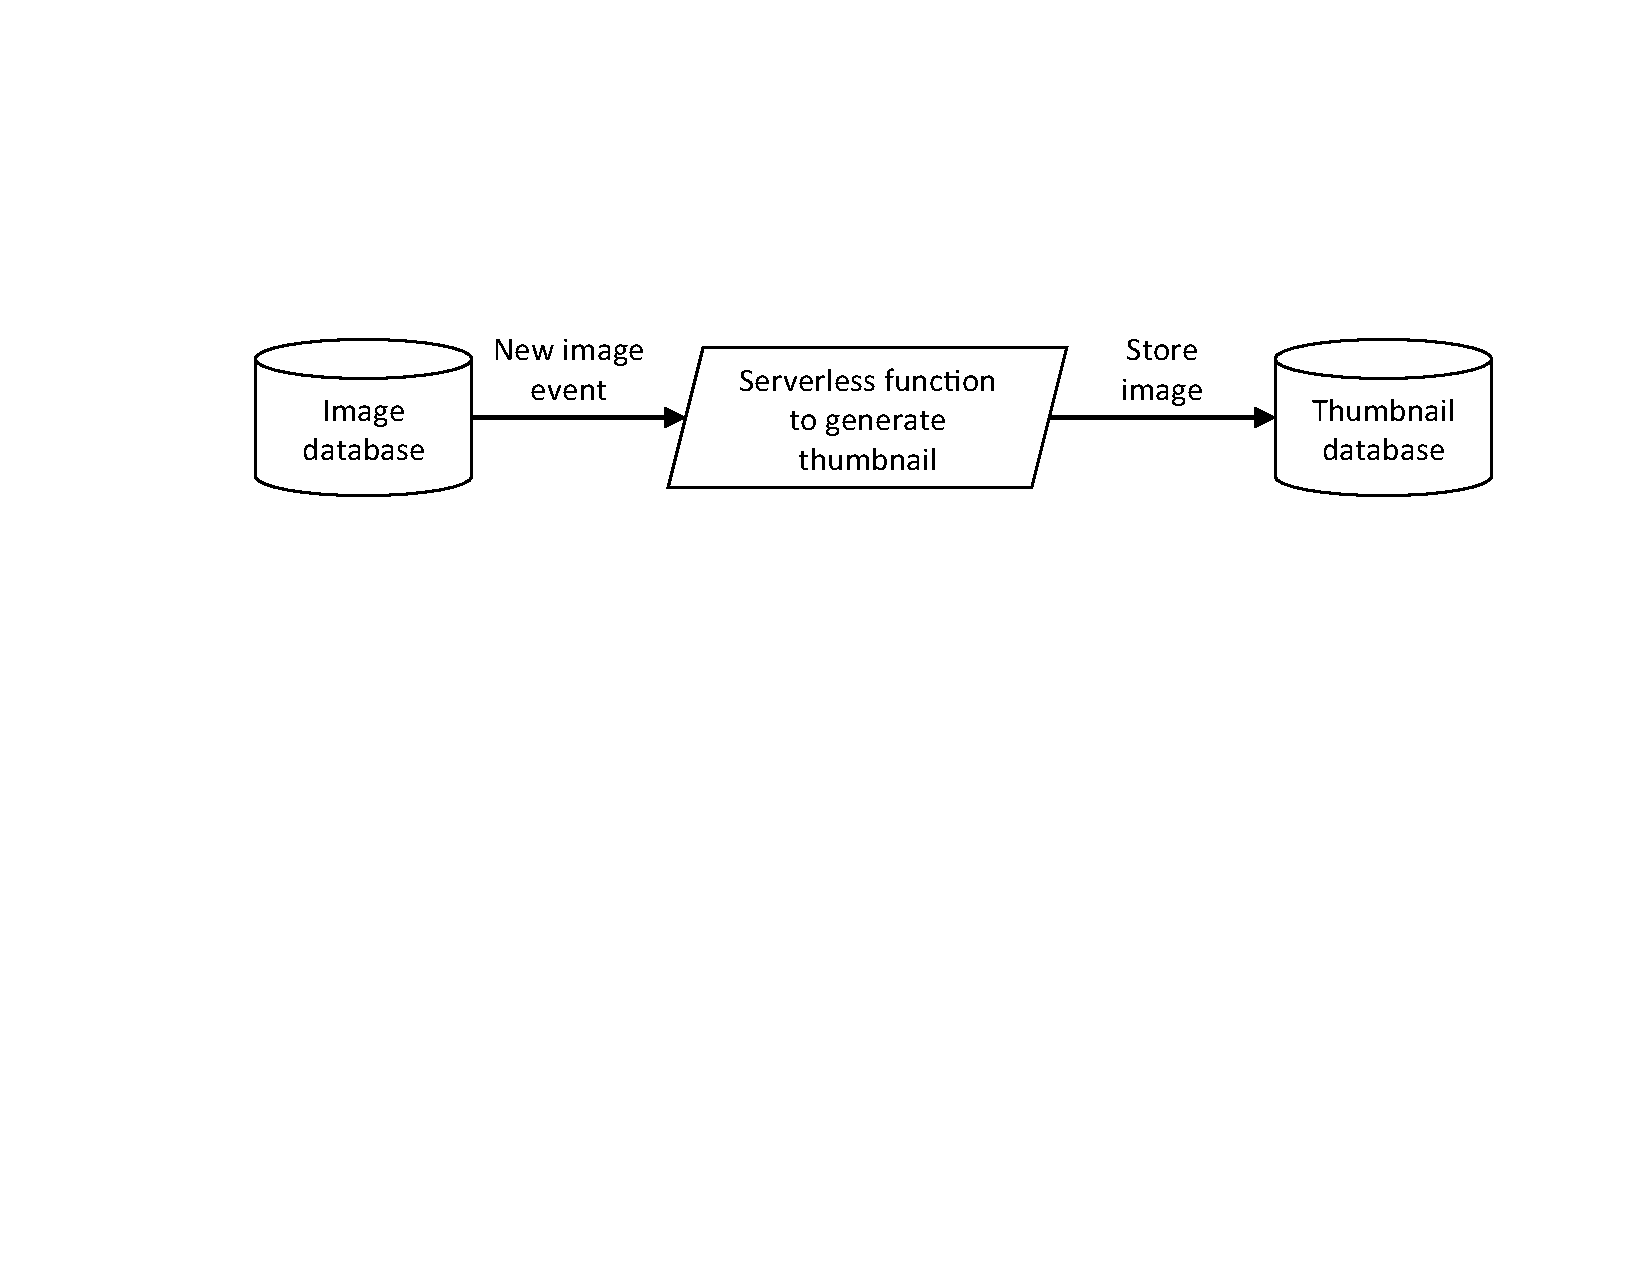
\includegraphics[width=\textwidth]{UseCase-Thumbnail2}
\caption{Image processing}
\label{fig:UseCase-Thumbnail}
\end{figure*}


In this tutorial, we will present serverless computing, survey existing serverless platforms from industry, academia, and open source projects, identify key characteristics and use cases, and  describe technical challenges and open problems. Our tutorial will involve a hands-on experience of using the serverless technologies available from different cloud providers (e.g. IBM, Amazon, Google and Microsoft). We expect our users to have basic knowledge of programming and basic knowledge of cloud computing.


Serverless computing is still in its infancy, hence it should be of interest to the ICDCS community, because there an opportunity for researchers to understand it and shape it by addressing the challenges that it faces. We hope that this tutorial (along with the first ICDCS workshop on serverless computing WoSC 2017) provides the first steps in understanding the technology and architecture of Serverless computing.






\section{Biography}
{\noindent \bf Paul Castro, Ph.D.}: is a Research Staff Member at the IBM Watson Research Center. He has been active in research on mobile and pervasive computing, cloud infrastructure, wireless location systems, location databases, stream processing, and enterprise web applications and has been awarded several patents in these areas. He has worked on cloud services for supporting mobile applications running on various smart phone platforms. Work from his research in the area of multi-device application support was recently released as part of the IBM Bluemix Mobile Backend as a Service. He has earned two IBM Technical Achievement Awards for the IBM SmartCloud Web Meetings for mobile clients and the Intelligent Notification System. Most recently, he worked on Apache OpenWhisk for Bluemix, with a focus on mobile solutions.

\smallbreak

{\noindent \bf Vatche Ishakian}: is an Assistant Professor in the Computer Information Systems department at Bentley University. He completed his PhD in Computer Science from Boston University. His research interests include distributed systems, process analytics, and priced based models for cloud services. Before embarking on an his academic career, Vatche was a Research Staff Member at IBM Research working on several projects including Apache OpenWhisk serverless computing platform.

\smallbreak

{\noindent \bf Vinod Muthusamy}: is a Research Staff Member in the Cognitive Cloud group at the IBM T.J. Watson Research Center. He completed his PhD in Computer Engineering at the University of Toronto. Vinod's research interests include publish/subscribe event processing, process analytics, machine learning in the cloud, and serverless computing. Most recently, he worked on Apache OpenWhisk Serverless Computing platform.

\smallbreak

{\noindent \bf Aleksander Slominski}: is a Research Staff Member in the Services and API Ecosystems Group at the IBM T.J. Watson Research Center. He is interested in development of applications for for future API Economy that take advantage of upcoming cloud programming approaches, such as serverless computing, for compositions and orchestration of components into business workflows. Most recently, he worked on Apache OpenWhisk Serverless Computing platform.

% references section
\nocite{*}


\bibliographystyle{IEEEtran}
% argument is your BibTeX string definitions and bibliography database(s)
\bibliography{references}
%


% that's all folks
\end{document}
